% Insert in a two-column A4 report with \usepackage{graphicx}.
% Designed for a full-width 178 mm figure, not an 85 mm single column.
% Adjust the path if the report build directory differs.
\begin{figure*}[t]
\centering
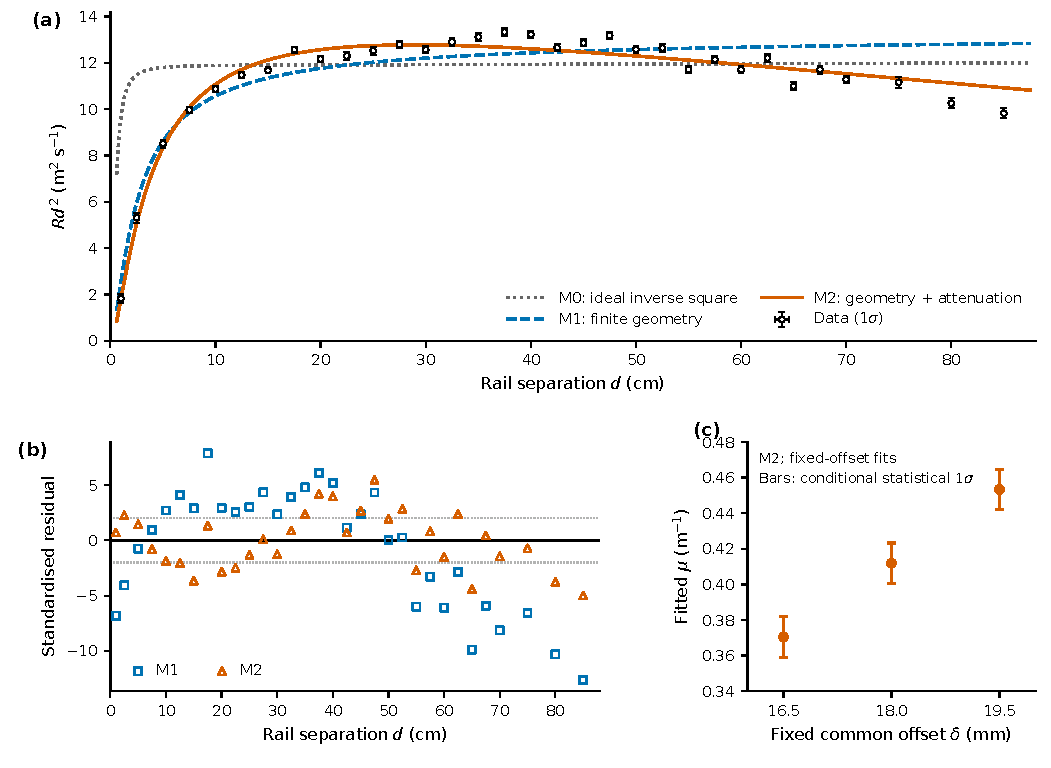
\includegraphics[width=178mm]{../results/figures/final_three_panel.pdf}
\caption{Testing geometric and effective-attenuation explanations of the
$^{90}$Sr/$^{90}$Y distance scan. (a) All 32 observed count rates multiplied by
rail separation squared, with propagated Poisson and independent reading
$1\sigma$ errors, and common-response M0--M2 fits. Horizontal and vertical
reading-error contributions are correlated. (b) M1/M2 residuals
$[n_i/t_i-\widehat R(d_i)]/[\widehat R(d_i)/t_i+
(s_i\widehat R'(d_i))^2]^{1/2}$; the zero and $\pm2$ lines are guides.
This diagnostic omits shared offset, background and fitted-parameter
covariance and model uncertainty, so residuals are not independent
significance tests. (c) M2 refits at three fixed common offsets; bars are
conditional local statistical $1\sigma$ at fixed offset and dead time.
The scenario span is not a confidence interval. All models use the same
background control and fixed dead-time response. M2 improves total deviance
but retains substantial lack of fit ($216.6/30$); its $\mu$ is a
phenomenological coefficient, not a measured air absorption coefficient.}
\label{fig:sr90-three-models}
\end{figure*}
